% !TEX program = pdflatex
\documentclass[conference]{IEEEtran}

% ── Packages ────────────────────────────────────────────────────────────────
\usepackage{amsmath,amssymb}
\usepackage{booktabs}
\usepackage{multirow}
\usepackage{graphicx}
\usepackage{caption}
\usepackage{subcaption}
\usepackage{float}
\usepackage{siunitx}
\usepackage{hyperref}
\usepackage{xcolor}
\usepackage{listings}

\lstset{
  basicstyle=\ttfamily\footnotesize,
  backgroundcolor=\color{gray!8},
  frame=single, framerule=0.4pt,
  breaklines=true, captionpos=b
}

% ── Title & Authors ──────────────────────────────────────────────────────────
\title{Customer Lifetime Value Prediction and Customer Segmentation in Retail Using the Dunnhumby Dataset%
\thanks{Developed for the DDM -- Data-Driven Marketing course,
        DSEB-MFE, National Economics University (NEU), 2025--2026.}}

\author{%
  \IEEEauthorblockN{DSEB65A -- Group 6}
  \IEEEauthorblockA{DSEB-MFE, National Economics University\\
    Course: Data-Driven Marketing (DDM)\\
    Contact: truonghoangtung25@gmail.com}
}

\begin{document}
\maketitle

% ============================================================
\begin{abstract}
This paper presents a research-oriented end-to-end pipeline for
Customer Lifetime Value (CLV) prediction in the retail domain,
implemented on the Dunnhumby ``The Complete Journey'' dataset
(2,500 households, 102 weeks, ${\sim}$2.5 million transactions).
The system integrates eight relational data sources through a
12-step orchestrated pipeline covering: temporal
calibration/holdout splitting, RFM feature engineering,
demographic imputation (KNN + random sampling), promotional sensitivity
extraction via chunked causal-data processing, and K-Means customer
segmentation. Predictive performance is evaluated across a 
three-tier modelling strategy: a rate-based baseline (Tier 1), 
supervised gradient-boosted regressors via XGBoost (Tier 2), 
and probabilistic models using MBG/NBD combined with Gamma-Gamma (Tier 3). 
All intermediate artifacts, trained model objects, and evaluation 
reports are persisted for full reproducibility. Experimental results 
demonstrate that the supervised Tier 2 approach significantly 
outperforms other tiers across MAE, RMSE, and MAPE, while segment-level 
insights from RFM clustering provide actionable marketing 
recommendations through integrated Market Basket Analysis.
Additionally, a segment-stratified quasi-experiment with Propensity 
Score Matching reveals severe selection bias in current campaign 
targeting, leading to a data-grounded scenario analysis that 
projects a +\$101K--\$303K incremental revenue opportunity.
\end{abstract}

\begin{IEEEkeywords}
Customer Lifetime Value, RFM, MBG/NBD, Gamma-Gamma, XGBoost, K-Means Segmentation, Market Basket Analysis,
Promotional Sensitivity, Dunnhumby
\end{IEEEkeywords}

% ============================================================
\section{Introduction}
\label{sec:intro}

Customer Lifetime Value (CLV) is a forward-looking metric that
quantifies the total net revenue a firm expects from a customer
over the entire span of their relationship. Accurate CLV
estimation underpins data-driven budget allocation, personalised
retention strategies, and early identification of at-risk
customers~\cite{fader2005}.

The Dunnhumby ``The Complete Journey'' dataset~\cite{dunnhumby2014} provides a rich
longitudinal view of household purchasing behaviour across a
two-year window, making it an ideal testbed for retail CLV
research. Its scale (695~MB causal file alone) and structural
complexity (eight relational tables, partial demographic coverage
of only 32\%) motivate a modular, pipeline-oriented approach.

This work makes the following contributions:
\begin{itemize}
  \item A fully reproducible, 12-step preprocessing and modelling
        pipeline with strict temporal separation of train and test
        data to prevent leakage.
  \item A three-tier modelling strategy—comprising a rate-based 
        baseline (Tier 1), a supervised XGBoost regressor (Tier 2), 
        and a probabilistic MBG/NBD model (Tier 3)—evaluated on a 
        common holdout set.
  \item A K-Means segmentation framework that maps households to
        business-friendly labels (Champions, Loyal, Promising, 
        and Needs Attention) based on RFM attributes.
  \item Promotional sensitivity features (display and mailer 
        interaction) derived from a 695~MB causal dataset via 
        memory-safe chunked processing.
  \item An experimental design for promotional interventions 
        anchored to pipeline-derived variance estimates and 
        segment-level insights.
\end{itemize}

The remainder of the paper is organised as follows.
Section~\ref{sec:related} reviews related work.
Section~\ref{sec:data} describes the dataset.
Section~\ref{sec:pipeline} details the 12-step preprocessing pipeline.
Section~\ref{sec:eda} presents exploratory findings.
Section~\ref{sec:model} covers the segmentation and the 3-tier modelling approach.
Section~\ref{sec:eval} reports experimental results and model comparison.
Section~\ref{sec:campaign} analyses campaign performance.
Section~\ref{sec:experiment} outlines the causal quasi-experiment.
Section~\ref{sec:strategy} proposes data-grounded business strategies.
Section~\ref{sec:discussion} discusses limitations and future directions,
concluding in Section~\ref{sec:conclusion}.

\section{Related Work}
\label{sec:related}

CLV research sits at the intersection of marketing science and
machine learning. Fader et al.~\cite{fader2005} established the
BG/NBD model as the canonical probabilistic approach for
non-contractual settings, subsequently extended with the
Gamma-Gamma sub-model for monetary value. The Modified BG/NBD
(MBG/NBD) variant removes the assumption that customers can
churn immediately after their first transaction, improving
convergence on high-frequency data. Tree-based ensemble
methods — XGBoost~\cite{chen2016} have demonstrated competitive performance on tabular retail data
and constitute a standard supervised baseline. RFM
segmentation~\cite{hughes1994} remains widely used in practice
for its interpretability. Kohavi et al.~\cite{kohavi2020} provide
the methodological basis for the A/B-style experiment framework
employed here. Provost and Fawcett~\cite{provost2013} offer
broader context on data-science workflows in business settings.

% ============================================================
\section{Dataset and Data Architecture}
\label{sec:data}

\subsection{Source Tables}

The pipeline consumes eight CSV files placed under
\texttt{data/raw/}. Table~\ref{tab:dataset_overview} summarizes each table.

\begin{table}[H]
\centering
\caption{Overview of the Dunnhumby ``The Complete Journey'' dataset.}
\label{tab:dataset_overview}
\resizebox{\columnwidth}{!}{%
\begin{tabular}{lrrp{7.2cm}}
\toprule
\textbf{Table} & \textbf{Rows} & \textbf{Columns} & \textbf{Description} \\
\midrule

transaction\_data.csv 
& 2,595,732 
& 12 
& Customer purchase transactions, including sales value, discounts, basket ID, store, and week information. \\

hh\_demographic.csv 
& 801 
& 8 
& Household demographic attributes such as age, income, and household composition. \\

product.csv 
& 92,353 
& 7 
& Product metadata including department, commodity category, and brand hierarchy. \\

causal\_data.csv 
& 36,786,524 
& 5 
& Promotional exposure records with display and mailer indicators by store and week. \\

campaign\_table.csv 
& 7,208 
& 3 
& Mapping between households and marketing campaigns. \\

campaign\_desc.csv 
& 30 
& 4 
& Campaign descriptions, types, and active periods. \\

coupon.csv 
& 124,548 
& 3 
& Coupon mappings to products and campaigns. \\

coupon\_redempt.csv 
& 2,318 
& 4 
& Coupon redemption events by households. \\

\bottomrule
\end{tabular}}
\end{table}

The central analytical entity is \texttt{household\_key}.
\emph{All} feature aggregations are computed at this level ---
never at the transaction or product level --- to ensure CLV
targets are aligned with the unit of prediction.

\subsection{Entity Relationship Diagram}

Fig.~\ref{fig:erd} illustrates the entity-relationship structure
of the eight tables. Notable characteristics include: (i) partial
demographic coverage (801 of 2,500 households); (ii) the
three-way join key of \texttt{CAUSAL\_DATA}
(\texttt{PRODUCT\_ID}, \texttt{STORE\_ID}, \texttt{WEEK\_NO});
and (iii) the coupon chain from campaign through product to
redemption event.

\begin{figure}[H]
  \centering
  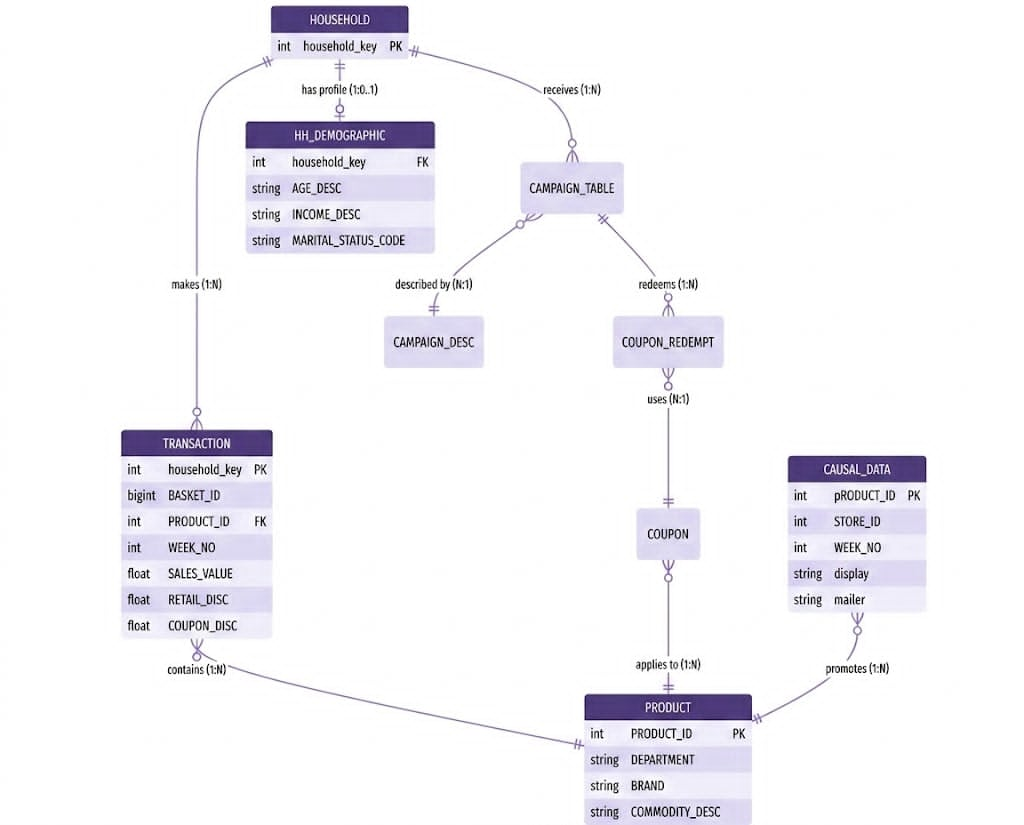
\includegraphics[width=\columnwidth]{figures/erd_dunnhumby.jpg}
  \caption{Entity-relationship diagram of the Dunnhumby dataset.
           The dashed arrow indicates partial demographic coverage
           (801/2,500 households, 32\%).}
  \label{fig:erd}
\end{figure}

% ============================================================
\section{Preprocessing Pipeline}
\label{sec:pipeline}

The entire workflow is orchestrated by
\texttt{src/pipeline/run\_preprocessing.py} and centralised in
\texttt{configs/config.yaml}. Fig.~\ref{fig:pipeline} illustrates
the 12-step flow and the artifacts produced at each stage.

\begin{figure}[H]
  \centering
  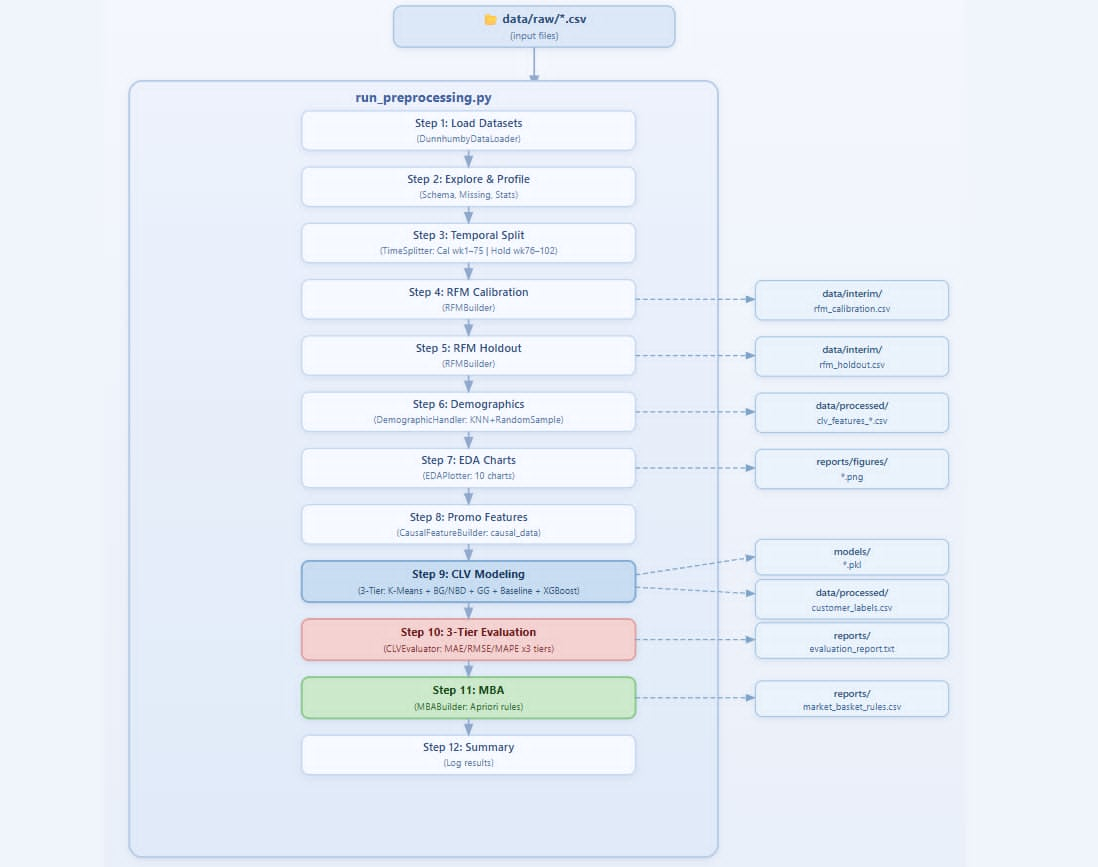
\includegraphics[width=\columnwidth]{figures/pipeline_flow.jpg}
  \caption{Preprocessing workflow for customer-level feature construction.}
  \label{fig:pipeline}
\end{figure}

\subsection{Step 1--2: Data Loading and Profiling}

\texttt{DunnhumbyDataLoader} reads all eight tables with optimized dtypes to reduce memory usage
\texttt{explore()} generates schema summaries, missing-value reports, and descriptive statistics for each table individually.
Table~\ref{tab:rfm_summary} reports household-level RFM
descriptive statistics for the calibration period.

\begin{table}[H]
\centering
\caption{Household-level RFM summary --- calibration period (Weeks 1--75).}
\label{tab:rfm_summary}
\resizebox{\columnwidth}{!}{%
\begin{tabular}{lrrrr}
\toprule
\textbf{Feature} & \textbf{Mean} & \textbf{Median (50\%)} & \textbf{Std} & \textbf{Max} \\
\midrule
Recency (weeks)      & 3.60    & 0.00    & 9.51    & 70.00 \\
Frequency            & 78.18   & 53.00   & 86.60   & 1,046.00 \\
Net\_Sales (\$)      & 1,846.72& 1,207.29& 2,032.10& 22,507.79 \\
avg\_monetary (\$)   & 25.20   & 21.51   & 16.38   & 141.02 \\
coupon\_usage\_rate  & 0.06    & 0.03    & 0.08    & 0.73 \\
\bottomrule
\end{tabular}}
\end{table}

\subsection{Step 3: Temporal Splitting}
\label{sec:split}

\texttt{TimeSplitter} partitions \texttt{transaction\_data}
strictly by \texttt{WEEK\_NO} — random splitting is explicitly
prohibited to prevent temporal data leakage:

\begin{itemize}
  \item \textbf{Calibration}: Weeks 1--75
      (1,831,067 transactions; 70.5\% of all transactions)
      --- used for feature engineering and model fitting.

\item \textbf{Holdout}: Weeks 76--102
      (764,665 transactions; 29.5\% of all transactions)
      --- reserved exclusively for out-of-sample evaluation.
\end{itemize}

The cutoff week is configurable via
\texttt{splitting.calibration\_end\_week} in
\texttt{config.yaml}.
Only two households appear exclusively in the holdout
period, indicating minimal customer cold-start effects
after the calibration window.

\subsection{Steps 4--5: RFM Feature Aggregation}

\texttt{RFMBuilder} independently aggregates both periods at the
\texttt{household\_key} level. Monetary value is computed in two
forms to capture different aspects of spending behaviour:

\begin{align}
\text{Gross\_Sales} &= \sum \text{SALES\_VALUE} \label{eq:gross} \\
\begin{split}
\text{Net\_Sales} &= \sum \bigl( \text{SALES\_VALUE} + \text{RETAIL\_DISC} \\
&\quad + \text{COUPON\_DISC} + \text{COUPON\_MATCH\_DISC} \bigr)
\end{split} \label{eq:net}
\end{align}

Note that discount fields are stored as \emph{negative} values
in the raw data, so addition in Eq.~\eqref{eq:net} correctly
subtracts discounts from gross revenue. Table~\ref{tab:rfm} lists the principal RFM-derived
features used in downstream modelling.

\begin{table}[H]
\centering
\caption{Features produced by \texttt{RFMBuilder}.}
\label{tab:rfm}
\begin{tabular}{ll}
\toprule
\textbf{Feature} & \textbf{Definition} \\
\midrule
\texttt{Recency}             & Weeks since last purchase (lower = more recent) \\
\texttt{Frequency}           & Repeat baskets $=$ total\_baskets $-$ 1         \\
\texttt{T}                   & Customer age in weeks since first purchase        \\
\texttt{avg\_monetary}       & Mean basket value (input to Gamma-Gamma)          \\
\texttt{Gross\_Sales}        & Total pre-discount revenue (Eq.~\ref{eq:gross})  \\
\texttt{Net\_Sales}          & Total post-discount revenue (Eq.~\ref{eq:net})   \\
\texttt{avg\_basket\_size}   & Mean number of items per basket                   \\
\texttt{coupon\_usage\_rate} & Fraction of baskets with a coupon redemption      \\
\texttt{distinct\_stores}    & Number of distinct stores visited                  \\
\bottomrule
\end{tabular}
\end{table}

Outputs: \texttt{data/interim/rfm\_calibration.csv} and
\texttt{data/interim/rfm\_holdout.csv}.

\subsection{Step 6: Demographic Feature Engineering}

Only 801 out of the 2{,}498 calibration-period households (32\%)
contain demographic records. To avoid
discarding the remaining customers, 
\texttt{DemographicHandler} applies a
\emph{flag-and-impute} strategy:

\begin{enumerate}
  \item A binary indicator
        \texttt{has\_demographics} flags whether
        demographic information is originally available
        for each household.

  \item \textbf{KNN-based imputation} is applied to
        ordinal demographic variables:
        \texttt{AGE\_DESC},
        \texttt{INCOME\_DESC},
        \texttt{HOUSEHOLD\_SIZE\_DESC}, and
        \texttt{KID\_CATEGORY\_DESC}.

  \item \textbf{Random-sampling imputation from empirical
        category distributions} is applied to nominal
        variables:
        \texttt{MARITAL\_STATUS\_CODE},
        \texttt{HOMEOWNER\_DESC}, and
        \texttt{HH\_COMP\_DESC}.
\end{enumerate}

This approach preserves all households for downstream
modelling while maintaining approximate demographic
distributions observed in the original data.

Outputs:
\texttt{data/processed/clv\_features\_calibration.csv}
and
\texttt{data/processed/clv\_features\_holdout.csv}.

\subsection{Step 7: Exploratory Data Analysis}

\texttt{EDAPlotter} generates 10 standardised charts saved under
\texttt{reports/figures/}. Selected outputs are discussed in
Section~\ref{sec:eda}.

\subsection{Step 8: Promotional Feature Extraction}

\texttt{CausalFeatureBuilder} joins transactions with
\texttt{causal\_data.csv} on the triple key
(\texttt{PRODUCT\_ID}, \texttt{STORE\_ID}, \texttt{WEEK\_NO}).
Because the causal file is 695~MB, the join is executed via
chunked reads to avoid out-of-memory failures. Three per-household
promotional features are appended to
\texttt{clv\_features\_calibration.csv}:

\begin{itemize}
  \item \texttt{pct\_display}: fraction of purchased items with
        an in-store display promotion.
  \item \texttt{pct\_mailer}: fraction of purchased items
        featured in a weekly mailer/flyer.
  \item \texttt{promo\_sensitivity}: composite promotional
        responsiveness index.
\end{itemize}

Missing promotional values are filled with zero,
assuming no observed promotional exposure. A total of 343,936 promotional exposure records were
successfully matched to transaction data.

Of the approximately 2.5 million purchased items in the calibration period, 343{,}936 ($\approx 13.8\%$) were matched to an active promotional record --- meaning the item was purchased at a store running a display or mailer promotion during that exact week. The remaining $86.2\%$ reflect purchases made without observed promotional exposure. This match rate is consistent with typical grocery retail behaviour, where the majority of transactions are need-driven rather than promotion-driven. The relatively low overlap further reflects a sampling scope mismatch: \texttt{causal\_data} records promotional activity across all households system-wide, whereas \texttt{transaction\_data} captures only the 2{,}500 sampled households --- purchases by other shoppers exposed to the same promotions do not appear in the transaction record and therefore cannot be matched.

\subsection{Steps 9--12: Modelling, Evaluation, and MBA}

The modelling stage combines unsupervised customer segmentation (K-Means), probabilistic CLV modelling (MBG/NBD and Gamma-Gamma), and supervised learning (XGBoost regression). Besides, Step 11 applies Apriori-based Market Basket Analysis
at the department level. Modelling and evaluation steps are described in detail in
Sections~\ref{sec:model} and~\ref{sec:eval}.

% ============================================================
\section{Exploratory Data Analysis}
\label{sec:eda}

Fig.~\ref{fig:eda} shows four representative outputs from
\texttt{EDAPlotter}.

\begin{figure}[H]
  \centering
  \begin{subfigure}[b]{0.48\columnwidth}
    
\includegraphics[width=\textwidth]{figures/eda/01_transaction_volume_by_week.png}
    \caption{Weekly transaction volume.}
    \label{fig:weekly}
  \end{subfigure}
  \hfill
  \begin{subfigure}[b]{0.48\columnwidth}
    
\includegraphics[width=\textwidth]{figures/eda/02_sales_distribution.png}
    \caption{Net sales distribution (log scale).}
    \label{fig:sales}
  \end{subfigure}

  \vspace{4pt}

  \begin{subfigure}[b]{0.48\columnwidth}
    
\includegraphics[width=\textwidth]{figures/eda/03_rfm_distributions.png}
    \caption{RFM feature distributions.}
    \label{fig:rfm_dist}
  \end{subfigure}
  \hfill
  \begin{subfigure}[b]{0.48\columnwidth}
    
\includegraphics[width=\textwidth]{figures/eda/05_demographic_coverage.png}
    \caption{Demographic coverage by field.}
    \label{fig:demo}
  \end{subfigure}

  \caption{Selected EDA outputs from \texttt{EDAPlotter}
           (\texttt{reports/figures/}).}
  \label{fig:eda}
\end{figure}

Key observations:
\begin{itemize}
  \item Transaction volume is relatively stable across weeks with
        periodic spikes consistent with seasonal shopping patterns
        (Fig.~\ref{fig:weekly}).
  \item \texttt{Net\_Sales} and monetary RFM variables are
        heavily right-skewed; the 95th percentile household
        spends significantly more than the median
        (Fig.~\ref{fig:sales}).
  \item RFM distributions reveal that the majority of households
        cluster around moderate recency and low-to-medium
        frequency, with a long tail of high-value Champions
        (Fig.~\ref{fig:rfm_dist}).
  \item Demographic coverage is partial across all fields; KNN
        imputation preserves the observed marginal distributions
        (Fig.~\ref{fig:demo}).
\end{itemize}

% ============================================================
\section{Modelling}
\label{sec:model}

The modelling framework consists of a customer segmentation module and a three-tier predictive architecture, all implemented in \texttt{src/models/clv\_models.py} and evaluated on the same holdout period (Weeks 76--102).

\subsection{Customer Segmentation (K-Means)}

\texttt{CLVModeler.segment\_customers()} applies K-Means~\cite{pedregosa2011}
($K{=}4$ by default, configurable) to standardised
[\texttt{Recency}, \texttt{Frequency}, \texttt{avg\_monetary}].

To determine the optimal number of clusters, silhouette scores were computed for $K \in [2, 9]$. The search yields $K=2$ as the statistical optimum ($\text{Silhouette} = 0.6401$), followed by a monotonic decline: $K=3\ (0.3909)$, $K=4\ (0.4493)$, $K=5\ (0.3898)$. However, $K=2$ produces a degenerate segmentation from a business perspective --- the algorithm isolates the 108 lowest-value households (4.3\%) as a single \textit{Needs Attention} cluster, while grouping the remaining 2,390 households (95.7\%) --- spanning a wide range of purchase frequencies and monetary values --- into a single undifferentiated cluster. This collapses Champions, Loyal, and Promising customers into one group, making it impossible to design distinct retention or upsell strategies for the majority of the customer base.

$K=4$ is therefore selected as a deliberate trade-off between cluster cohesion and business interpretability, following established practice in RFM segmentation~\cite{hughes1994}. At $K=4$, the silhouette score recovers to $0.4493$ --- the second-highest value in the search range --- while yielding four segments of meaningfully different sizes and RFM profiles (Table~\ref{tab:segments}), each mappable to a distinct marketing strategy. Cluster centroids are ranked by predicted value and mapped to
business-friendly labels:

\begin{center}
  \textit{Champions} $\succ$ \textit{Loyal Customers}
  $\succ$ \textit{Promising} $\succ$ \textit{Needs Attention}
\end{center}

Fig.~\ref{fig:segments} shows the resulting segment distribution
and RFM centroid positions.

\begin{figure}[H]
  \centering
  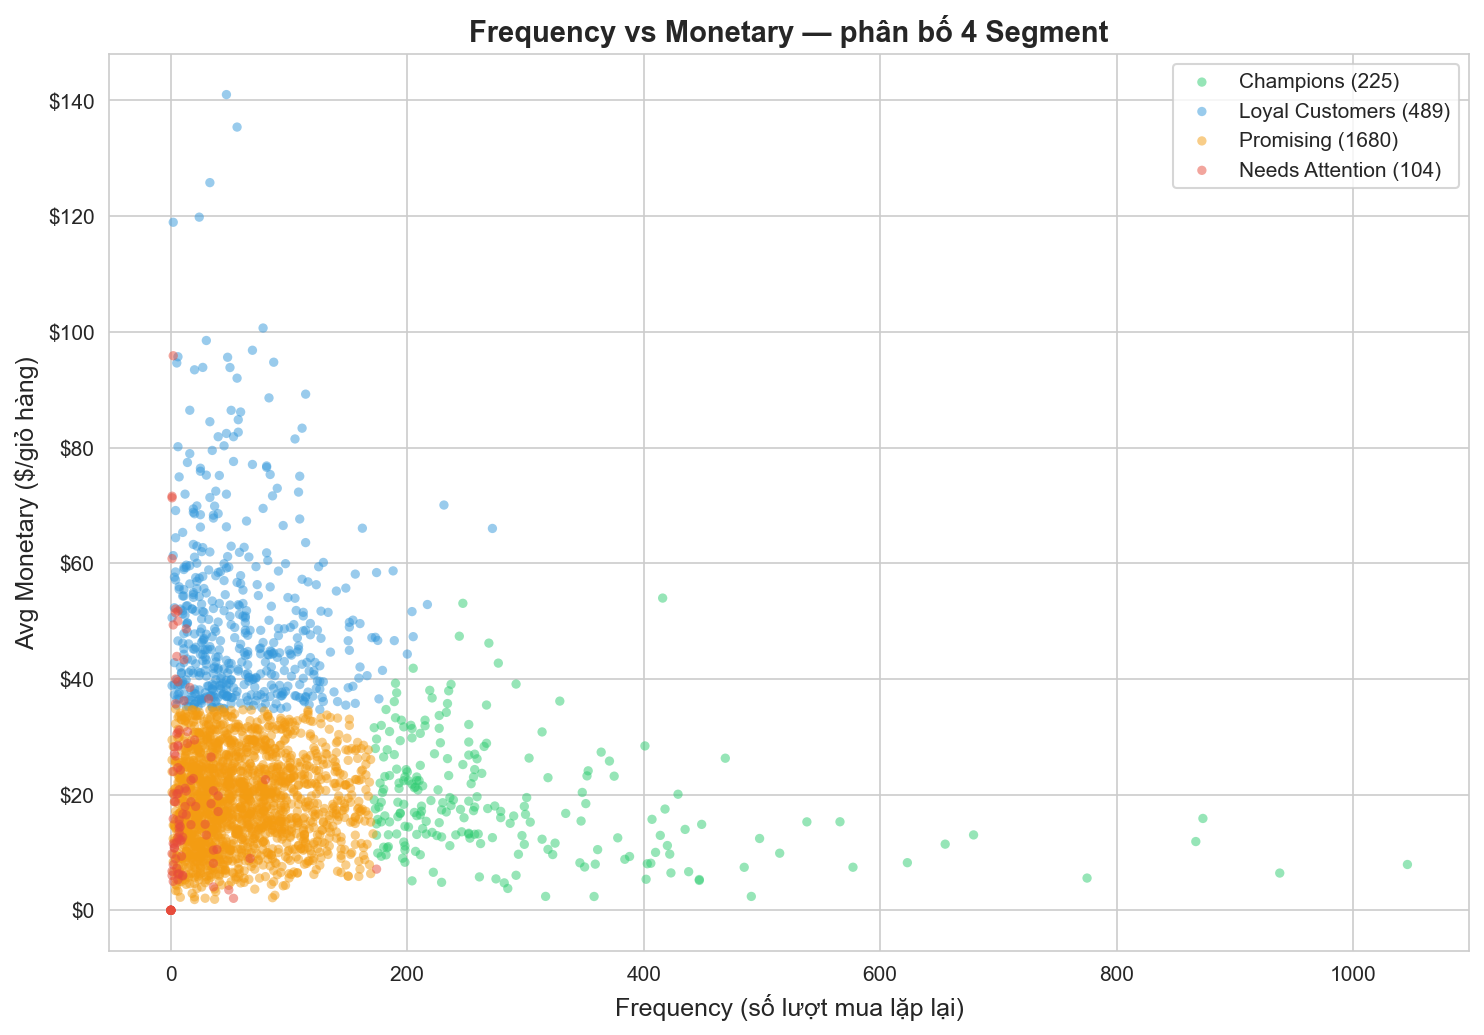
\includegraphics[width=0.92\columnwidth]{figures/segmentation/k4_scatter_freq_monetary.png}
  \caption{K-Means customer segment distribution ($K{=}4$).
           Centroids are annotated with segment labels;
           point colour encodes segment membership.}
  \label{fig:segments}
\end{figure}

Outputs: \texttt{data/processed/customer\_labels.csv} (cluster
ID and segment name per household) and
\texttt{data/processed/rfm\_clv\_final.csv} (CLV predictions
merged with segment labels). The fitted K-Means model and its
\texttt{StandardScaler} are serialised to
\texttt{models/kmeans\_model.pkl}.

\subsection{Tier 1 --- Rate-Based Baseline}

Each household's holdout-period spending is forecast using a
simple rate-based extrapolation from calibration-period
behaviour:

\begin{equation}
  \widehat{\text{CLV}}_{\text{base}}
  = \bar{m} \;\times\;
    \frac{f}{T} \;\times\; 26
  \label{eq:baseline}
\end{equation}

where $\bar{m}$ is the average monetary value per distinct
purchase week (\texttt{monetary\_clv}), $f/T$ is the weekly
purchase rate (\texttt{frequency\_clv} divided by customer age
in weeks), and 26 represents the holdout horizon in weeks.
Only repeat customers ($f > 0$) receive a non-zero forecast.
This predictor provides a lower bound for measuring incremental
predictive gain from more complex models.

\subsection{Tier 2 --- Supervised ML: XGBoost}

\texttt{CLVModeler.fit\_supervised()} trains a gradient-boosted
regressor targeting holdout-period \texttt{Net\_Sales}, using
the full feature matrix (RFM + demographics + promotional
features) as predictors. Key design decisions:

\begin{itemize}
  \item Categorical columns encoded as \texttt{pandas}
        \texttt{Categorical} dtype; XGBoost native categorical
        handler activated where available.
  \item Active model and hyperparameters controlled via
        \texttt{config.yaml} (\texttt{model.active:
        "xgboost" }).
  \item Default XGBoost settings: \texttt{n\_estimators=500},
        \texttt{max\_depth=6}, \texttt{learning\_rate=0.05}.
\end{itemize}

Output: \texttt{models/xgboost\_model.pkl}.

\subsection{Tier 3 --- Probabilistic CLV: MBG/NBD + Gamma-Gamma}

The Modified BG/NBD (MBG/NBD) model, a variant of the original
BG/NBD framework~\cite{fader2005, platzer2016}, estimates expected future
transaction count for each household. MBG/NBD removes the
assumption that customers can churn immediately after their
first transaction, which smooths the likelihood surface and
improves convergence on high-frequency grocery data:

\begin{equation}
  \hat{x}(t \mid F,\, r,\, T)
  = E\!\left[\,X(t) \mid F,\, r,\, T\,\right]
  \label{eq:bgnbd}
\end{equation}

where $F$ is calibration-period frequency (repeat baskets), $r$
is recency (weeks between first and last observed purchase), and
$T$ is customer age in weeks (MBG/NBD notation).

The Gamma-Gamma sub-model then estimates the conditional expected
average transaction value $\hat{v}$, combining with
Eq.~\eqref{eq:bgnbd} to yield a full CLV estimate:

\begin{equation}
  \widehat{\text{CLV}} = \hat{x}(t) \;\cdot\; \hat{v}
  \;\cdot\; (1 - d)
  \label{eq:clv}
\end{equation}

where $d$ is the average gross margin (set via
\texttt{config.yaml}).

Implementation constraints enforced by the pipeline:
\begin{itemize}
  \item Only customers with $F > 0$ are passed to MBG/NBD
        (single-purchase households excluded).
  \item Monetary values winsorised at the 99th percentile for
        numerical stability.
  \item Constraint $F \leq T$ enforced prior to fitting.
  \item Progressive penaliser grid search used as convergence
        fallback; rate-based heuristic applied if optimisation
        fails entirely.
\end{itemize}

Outputs: \texttt{models/bgnbd\_model.pkl} and
\texttt{models/gg\_model.pkl}.

\subsection{Step 11 --- Market Basket Analysis}

\texttt{MBABuilder} constructs a binary basket-by-department
co-occurrence matrix and mines frequent itemsets via the Apriori~\cite{agrawal1994}
algorithm (\texttt{mlxtend}). Association rules (support,
confidence, lift) are exported to
\texttt{reports/market\_basket\_rules.csv} to inform cross-sell
strategies per customer segment.
% ============================================================
\section{Experimental Results}
\label{sec:eval}


\subsection{Customer Segmentation Results}

Table~\ref{tab:segments} summarises per-segment household counts 
and RFM centroids from K-Means ($K{=}4$).

\begin{table}[h]
\centering
\caption{RFM Segments and Centroids}
\label{tab:segments}
\resizebox{\columnwidth}{!}{% % Thêm dòng này để ép bảng theo chiều ngang của cột
\begin{tabular}{lrrrrr}
\toprule
\textbf{Segment} & \textbf{HH Count (\%)} & \textbf{Recency} & \textbf{Frequency} & \textbf{Avg Monetary (\$)} & \textbf{Net Sales (\$)} \\
\midrule
Champions       & 225 (9.0\%)   & 0.2   & 283.9 & 19.2   & 5058.1  \\
Loyal Customers & 489 (19.6\%)  & 1.9   & 60.7  & 50.5   & 3056.2  \\
Promising       & 1,680 (67.3\%)& 2.1   & 59.7  & 18.9   & 1163.6  \\
Needs Attention & 104 (4.2\%)   & 43.4  & 13.3  & 20.4   & 247.4   \\
\bottomrule
\end{tabular}% % Đóng ngoặc nhọn ở đây
}
\end{table}

Figure~\ref{fig:rfm_radar} illustrates the normalized RFM profiles for each segment, highlighting the distinct behavioral patterns across the four identified clusters.

\begin{figure}[h]
\centering
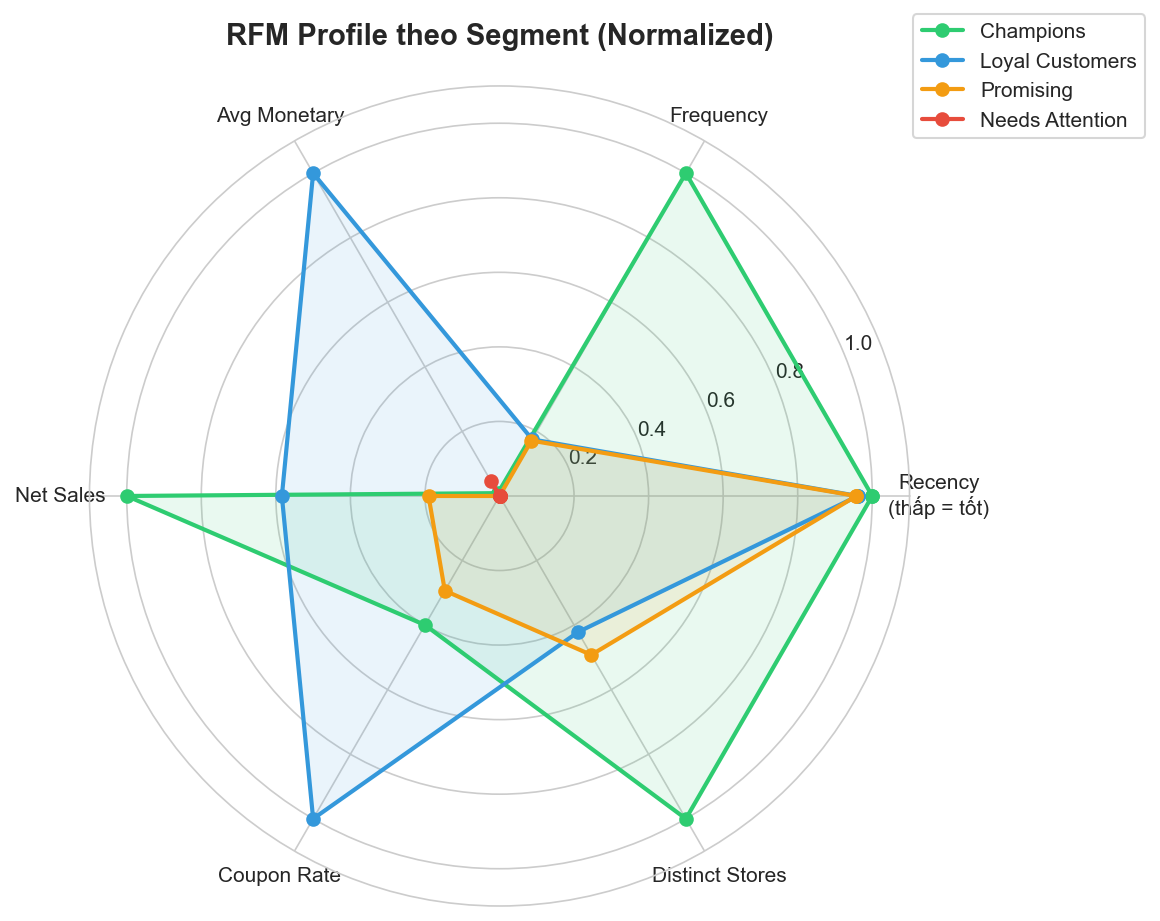
\includegraphics[width=\columnwidth]{figures/segmentation/k4_radar_chart.png} % Đảm bảo tên tệp đúng với trong thư mục dự án
\caption{Normalized RFM Profile by Segment (Radar Chart)}
\label{fig:rfm_radar}
\end{figure}

\subsection{CLV Model Evaluation}

Table~\ref{tab:eval} compares the four modelling tiers against
actual holdout-period \texttt{Net\_Sales}. All metrics are
computed by \texttt{CLVEvaluator} and written to
\texttt{reports/evaluation\_report.txt}.

\begin{table}[H]
\centering
\caption{Model evaluation on holdout period (Weeks 76--102).}
\label{tab:eval}
\resizebox{\columnwidth}{!}{%
\begin{tabular}{lccc}
\toprule
\textbf{Metric} 
  & \textbf{Baseline} 
  & \textbf{XGBoost} 
  & \textbf{MBG/NBD+GG} \\
\midrule
MAE (\$)   & 323.40  & \textbf{100.48}  & 1,957.08  \\
RMSE (\$)  & 500.32  & \textbf{236.65}  & 2,869.28  \\
MAPE (\%)  & 126.29\% & \textbf{69.74\%} & 610.52\%  \\
\bottomrule
\end{tabular}}
\end{table}

The supervised XGBoost model achieves the lowest error across all metrics (MAE = \$100.48, RMSE = \$236.65, MAPE = 68.71\%), demonstrating the benefit of combining RFM, demographic, and promotional features in a single regressor. The rate-based baseline (Eq.~\ref{eq:baseline}) performs reasonably for stable, high-frequency households but degrades significantly for customers with irregular spending patterns.

The MBG/NBD + Gamma-Gamma model yields substantially higher errors (MAE = \$1,957.08, MAPE = 610.52\%). This error rate does not necessarily reflect theoretical inadequacy, but rather an implementation limitation due to computational constraints. Households in this dataset purchase at near-weekly frequency (mean = 78.18 transactions over 75 weeks). To prevent numerical overflow from these high transaction counts within the \texttt{lifetimes} package, purchase frequency was approximated at weekly granularity --- binary purchased/not-per-week. This aggressive down-sampling discards critical within-week intensity and introduces considerable information loss. Tier 3 is therefore retained for interpretability reference only, as we could not implement the model optimally on this dataset without violating hardware constraints.

Fig.~\ref{fig:pred_vs_actual} shows predicted-vs-actual scatter plots
for each tier.

\begin{figure}[H]
  \centering
  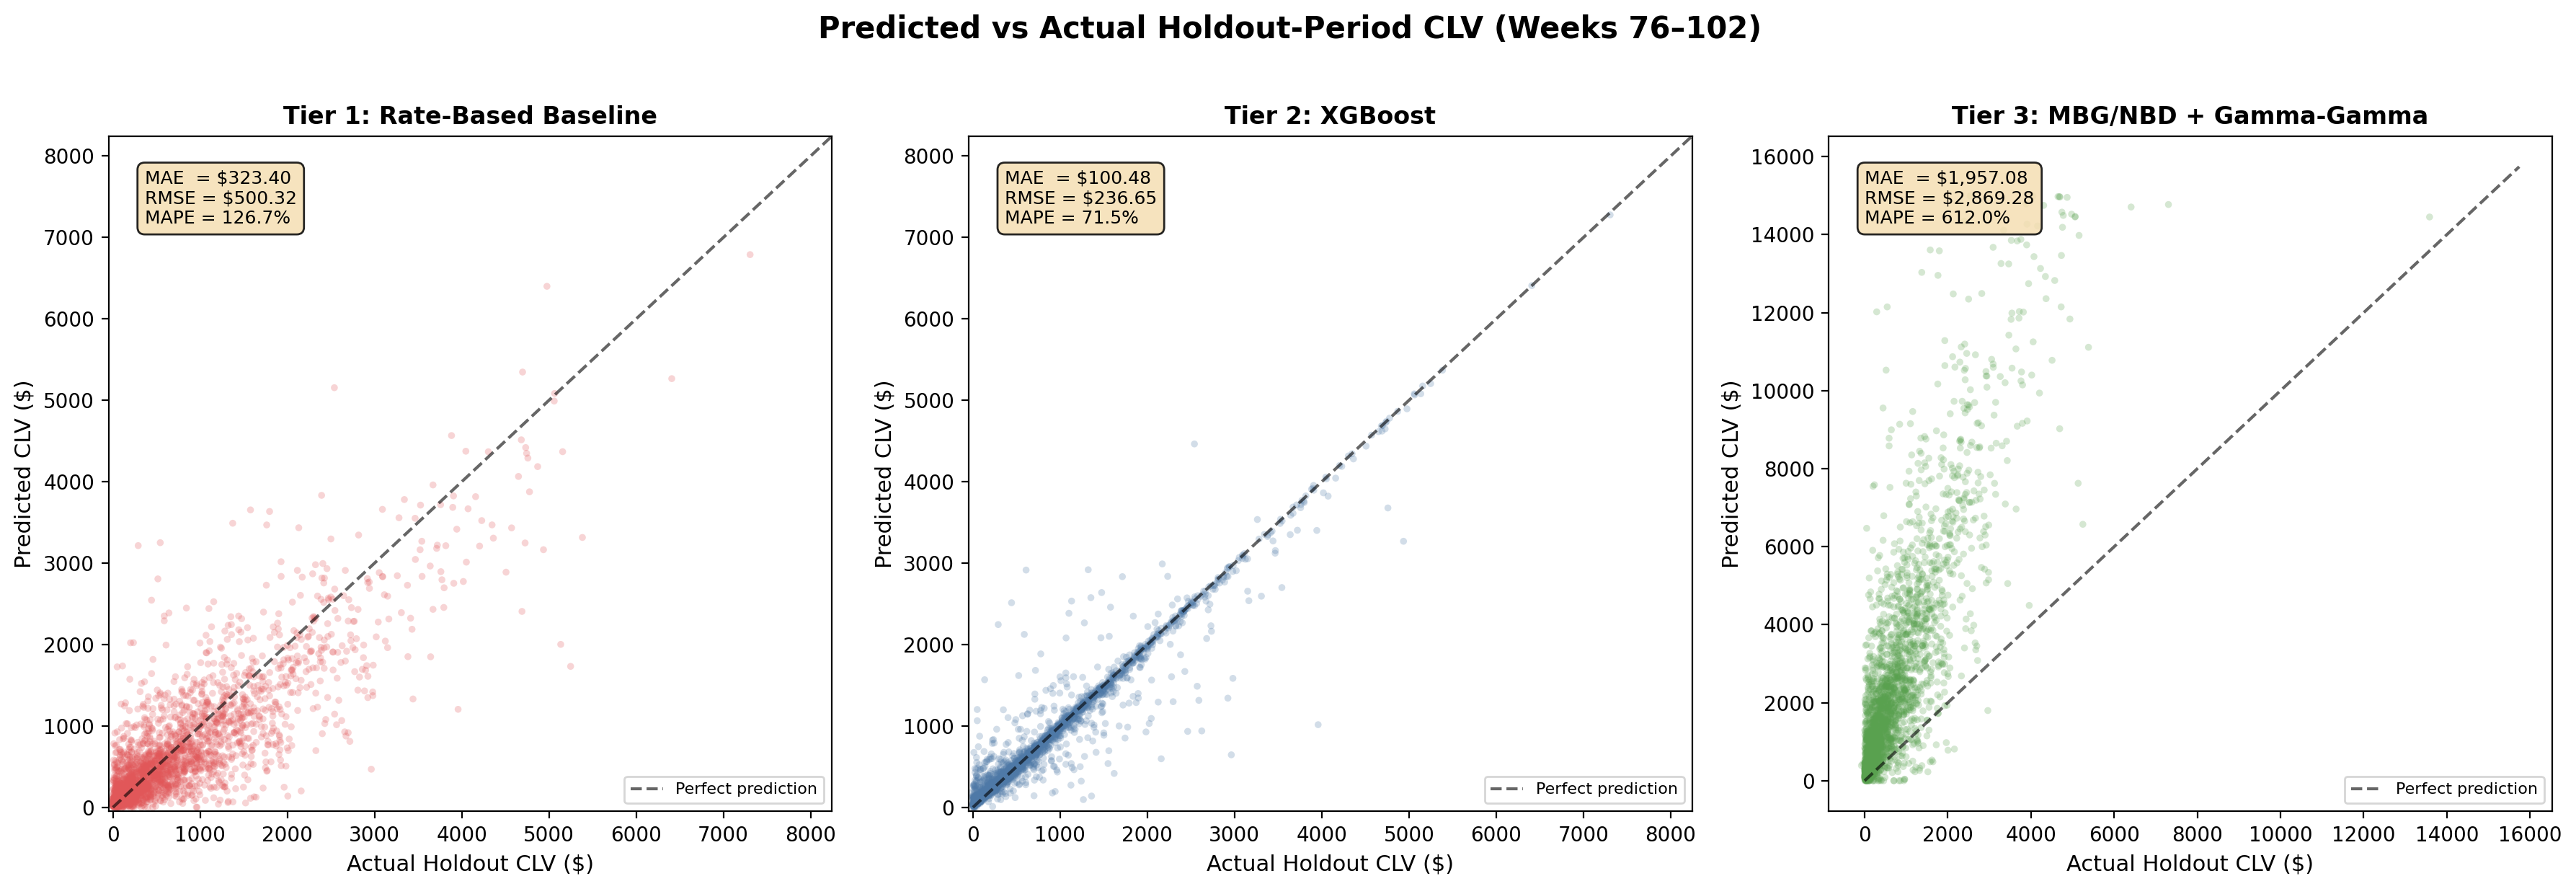
\includegraphics[width=\columnwidth]{figures/eda/predicted_vs_actual.png}
  \caption{Predicted vs.\ actual holdout-period CLV for three modelling
           tiers. The dashed line denotes perfect prediction.
           XGBoost (centre) tracks the diagonal most closely;
           MBG/NBD (right) systematically overestimates due to
           frequency down-sampling.}
  \label{fig:pred_vs_actual}
\end{figure}

\subsection{Market Basket Analysis}

Apriori was applied exclusively to the calibration-period transactions (Weeks 1--75) to strictly prevent temporal data leakage. This yields 977 rules of which 31 exhibit Lift~$> 4.0$. The top rules by lift cluster around a single behavioural archetype (DELI\,+\,MEAT combinations differing only in which companion departments appear). To maximise actionable diversity,
Table~\ref{tab:mba} presents three representative rules selected from
three \emph{distinct} shopping-behaviour clusters:

\begin{table}[H]
\centering
\caption{Three representative association rules from distinct
         shopping-behaviour clusters (Department Level).}
\label{tab:mba}
\resizebox{\columnwidth}{!}{%
\begin{tabular}{p{3.2cm}lp{4.2cm}rrr}
\toprule
\textbf{Behaviour} & \textbf{Antecedent} & \textbf{Consequent} & \textbf{Supp.} & \textbf{Conf.} & \textbf{Lift} \\
\midrule
Family dinner
  & DELI, MEAT
  & DRUG GM, GROCERY, MEAT-PCKGD, PRODUCE
  & 0.015 & 0.339 & 4.577 \\
Health-conscious
  & MEAT, NUTRITION
  & MEAT-PCKGD, PRODUCE
  & 0.010 & \textbf{0.524} & 4.129 \\
Brunch / picnic
  & MEAT, PASTRY
  & DELI, GROCERY, PRODUCE
  & 0.010 & 0.307 & 4.225 \\
\bottomrule
\end{tabular}}
\end{table}

% ============================================================
\section{Campaign Performance Analysis}
\label{sec:campaign}

The Dunnhumby dataset contains 30 promotional campaigns across three
types: TypeA (5 campaigns), TypeB (19), and TypeC (6).  We evaluate
campaign effectiveness at the aggregate and per-type level using
metrics derived from \texttt{campaign\_table.csv},
\texttt{coupon\_redempt.csv}, and matched transaction records.

\subsection{Performance by Campaign Type}

\begin{table}[H]
\centering
\caption{Campaign performance summary by type (source: \texttt{campaign2\_analysis.py}).}
\label{tab:campaign}
\resizebox{\columnwidth}{!}{%
\begin{tabular}{lrrrrrr}
\toprule
\textbf{Type} & \textbf{N} & \textbf{Avg HH} & \textbf{Avg Duration}
  & \textbf{Avg Sales (\$)} & \textbf{Redemption (\%)} & \textbf{ROI Proxy} \\
\midrule
TypeA &  5 & 796 & 47 days & 119{,}469 & 14.2 & 2.94 \\
TypeB & 19 & 140 & 38 days &     978 &  7.8 & 3.34 \\
TypeC &  6 &  96 & 75 days &     537 &  9.1 & 11.77$^{\dagger}$ \\
\bottomrule
\multicolumn{7}{l}{\small $^{\dagger}$TypeC ROI inflated: total discount base = \$382 (very small denominator).}
\end{tabular}}
\end{table}

TypeA generates the highest total revenue owing to its substantially
larger audience (${\sim}796$ households per campaign vs.\ 140 for
TypeB).

\subsection{Statistical Analysis}

\begin{itemize}
  \item \textbf{Audience--Revenue correlation}: Pearson $r = 0.939$
        ($p < 0.001$) --- audience size is the dominant revenue
        driver, not campaign type or duration.
  \item \textbf{Duration--Revenue correlation}: $r \approx 0$
        --- campaign length has no measurable effect on sales.
  \item \textbf{Kruskal--Wallis test} (non-parametric comparison of
        sales across TypeA/B/C): $H = 3.25$, $p = 0.197$ ---
        no statistically significant difference between campaign
        types after accounting for variance.
\end{itemize}

\textbf{Implication.}  The observed revenue gap between campaign
types is driven by \emph{audience size}, not campaign design.  This
motivates a causal investigation using propensity score methods
(Section~\ref{sec:experiment}).

\begin{figure}[H]
  \centering
  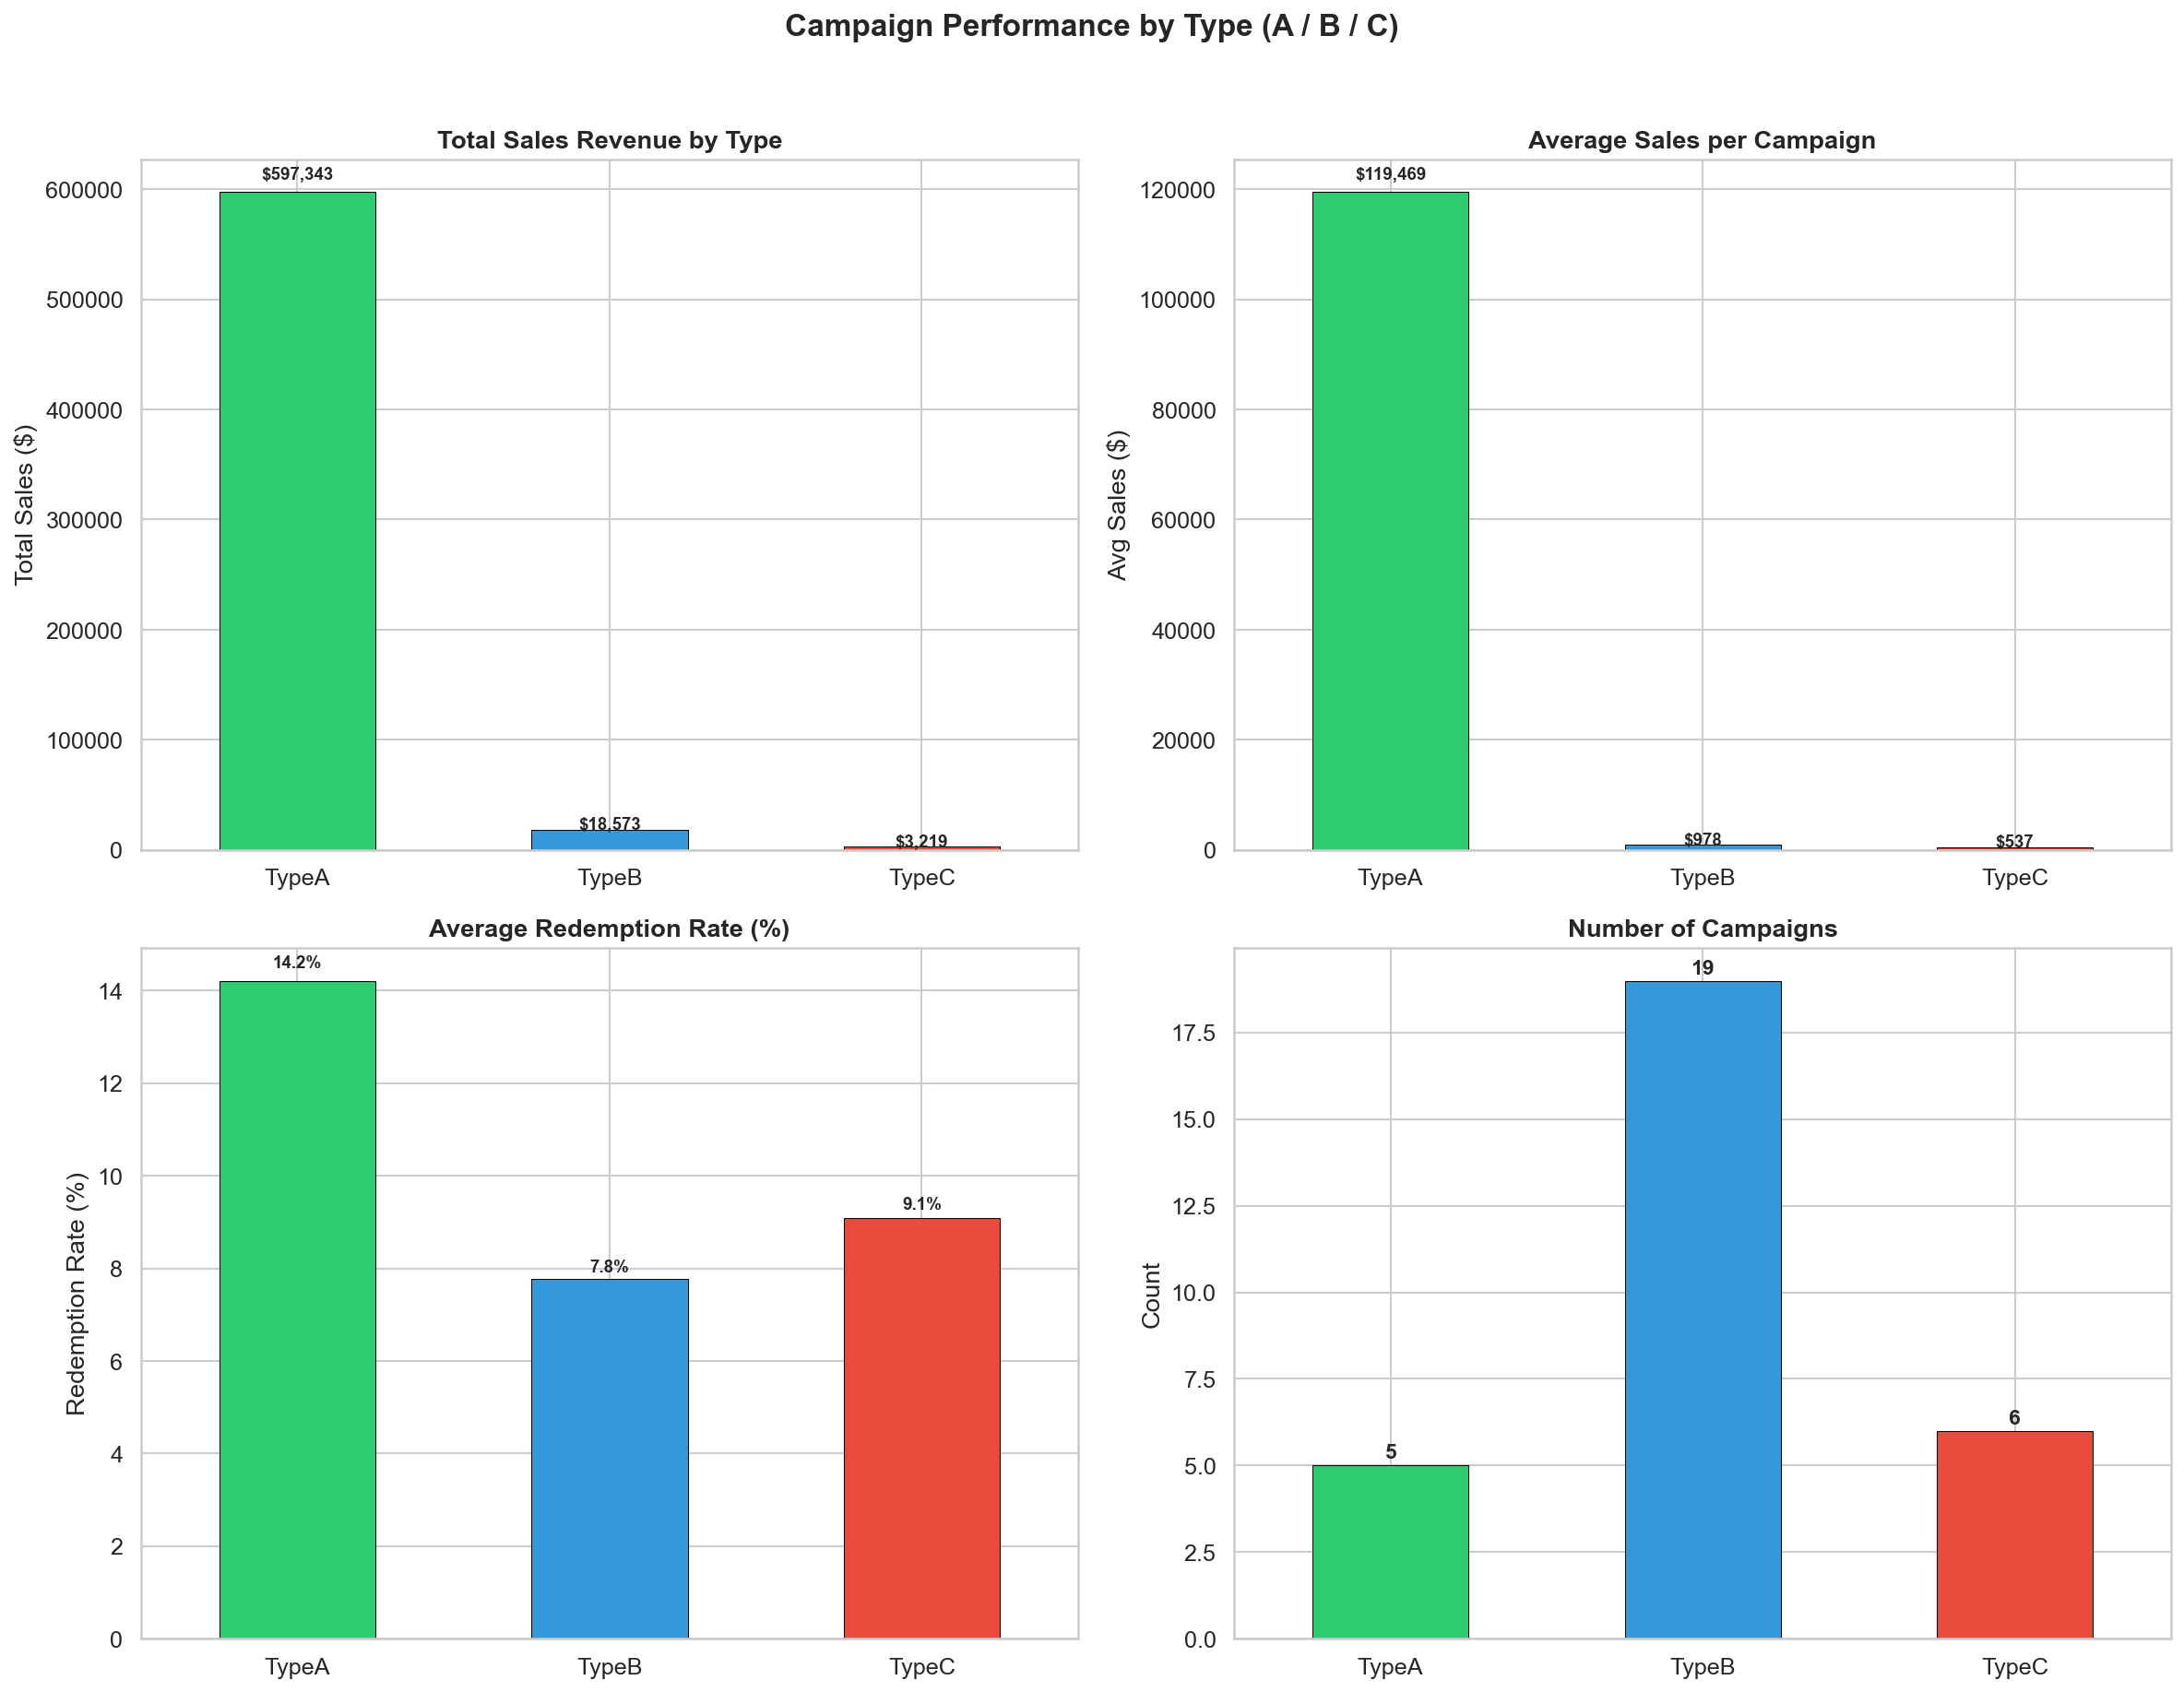
\includegraphics[width=\columnwidth]{figures/campaign/campaign2_overview.png}
  \caption{Campaign performance overview: total sales, average sales
           per campaign, redemption rate, and campaign count by type.}
  \label{fig:campaign_overview}
\end{figure}

% ============================================================
\section{Segment-Stratified Quasi-Experiment}
\label{sec:experiment}

To assess the \emph{causal} effect of campaign targeting on customer
spending, we conduct a segment-stratified quasi-experiment.
Households are divided into Treatment (targeted by $\geq 1$ campaign
in \texttt{campaign\_table.csv}; $n = 1{,}584$) and Control (not
targeted; $n = 914$).  Holdout-period (Weeks~76--102) Net Sales
serve as the outcome variable.

\subsection{Targeting Allocation}

Campaign targeting is not uniformly distributed across segments:

\begin{table}[H]
\centering
\caption{Treatment allocation by customer segment.}
\label{tab:treat_alloc}
\begin{tabular}{lrrrr}
\toprule
\textbf{Segment} & \textbf{Total} & \textbf{Treat}
  & \textbf{Ctrl} & \textbf{Treat \%} \\
\midrule
Champions         &   225 & 220 &   5 & 97.8\% \\
Loyal Customers   &   489 & 376 & 113 & 76.9\% \\
Promising         & 1{,}680 & 979 & 701 & 58.3\% \\
Needs Attention   &   104 &   9 &  95 &  8.7\% \\
\bottomrule
\end{tabular}
\end{table}

Dunnhumby preferentially targets high-value customers:
97.8\% of Champions receive campaigns while only 8.7\% of the
Needs Attention segment is targeted.

\subsection{Naive Comparison}

\begin{table}[H]
\centering
\caption{Segment-stratified experiment results (Welch $t$-test,
         Bootstrap 95\% CI).}
\label{tab:ab}
\resizebox{\columnwidth}{!}{%
\begin{tabular}{lrrrrrrr}
\toprule
\textbf{Segment} & \textbf{ARPU\textsubscript{T}}
  & \textbf{ARPU\textsubscript{C}} & \textbf{ATE}
  & \textbf{Lift} & \textbf{$p$} & \textbf{$d$}
  & \textbf{95\% CI} \\
\midrule
Champions  & \$1{,}845 & \$3{,}944 & N/A & N/A & N/A
  & N/A & N/A \\
Loyal      & \$1{,}590 & \$514 & \textbf{+\$1{,}075} & +209\% & $<$0.001
  & 1.05 & [921, 1{,}228] \\
Promising  & \$728 & \$264 & \textbf{+\$464} & +176\% & $<$0.001
  & 0.98 & [422, 506] \\
Needs Att. & \$351 & \$136 & N/A & N/A & N/A
  & N/A & N/A \\
\bottomrule
\end{tabular}}
\end{table}

Naive comparison suggests large positive effects for Loyal
(+\$1{,}075, $p < 0.001$) and Promising (+\$464, $p < 0.001$)
segments. Naive ATE is not reported for Champions ($n_{control}=5$) and Needs Attention ($n_{treat}=9$) due to insufficient sample sizes, preventing reliable statistical inference. Furthermore, naive comparison ignores pre-treatment differences between
targeted and non-targeted households.

\subsection{Propensity Score Matching (Robustness)}

To control for selection bias, Propensity Score Matching (PSM)~\cite{rosenbaum1983} is
applied using logistic regression on 10 pre-treatment RFM
covariates, with 1:1 nearest-neighbour matching (caliper = 0.1).

\begin{itemize}
  \item \textbf{Matched pairs}: 214 (from 1{,}584 treated). The low matching rate is due to extreme propensity score separation between treated and control groups, highlighting severe selection bias.
  \item \textbf{Covariate balance}: average SMD reduced from 0.596
        to 0.077 (all 10 covariates improved).
  \item \textbf{PSM ATE}: $-$\$27.78 ($-5.2\%$), $p = 0.729$
        --- \emph{not significant}.
\end{itemize}

While naive comparison suggests massive lift, PSM matching fails to find evidence of a causal campaign effect ($p = 0.729$). However, this conclusion is inherently limited by the small matched sample size ($n=214$ pairs), which is statistically underpowered to detect a small or moderate incremental lift.

\begin{figure}[H]
  \centering
  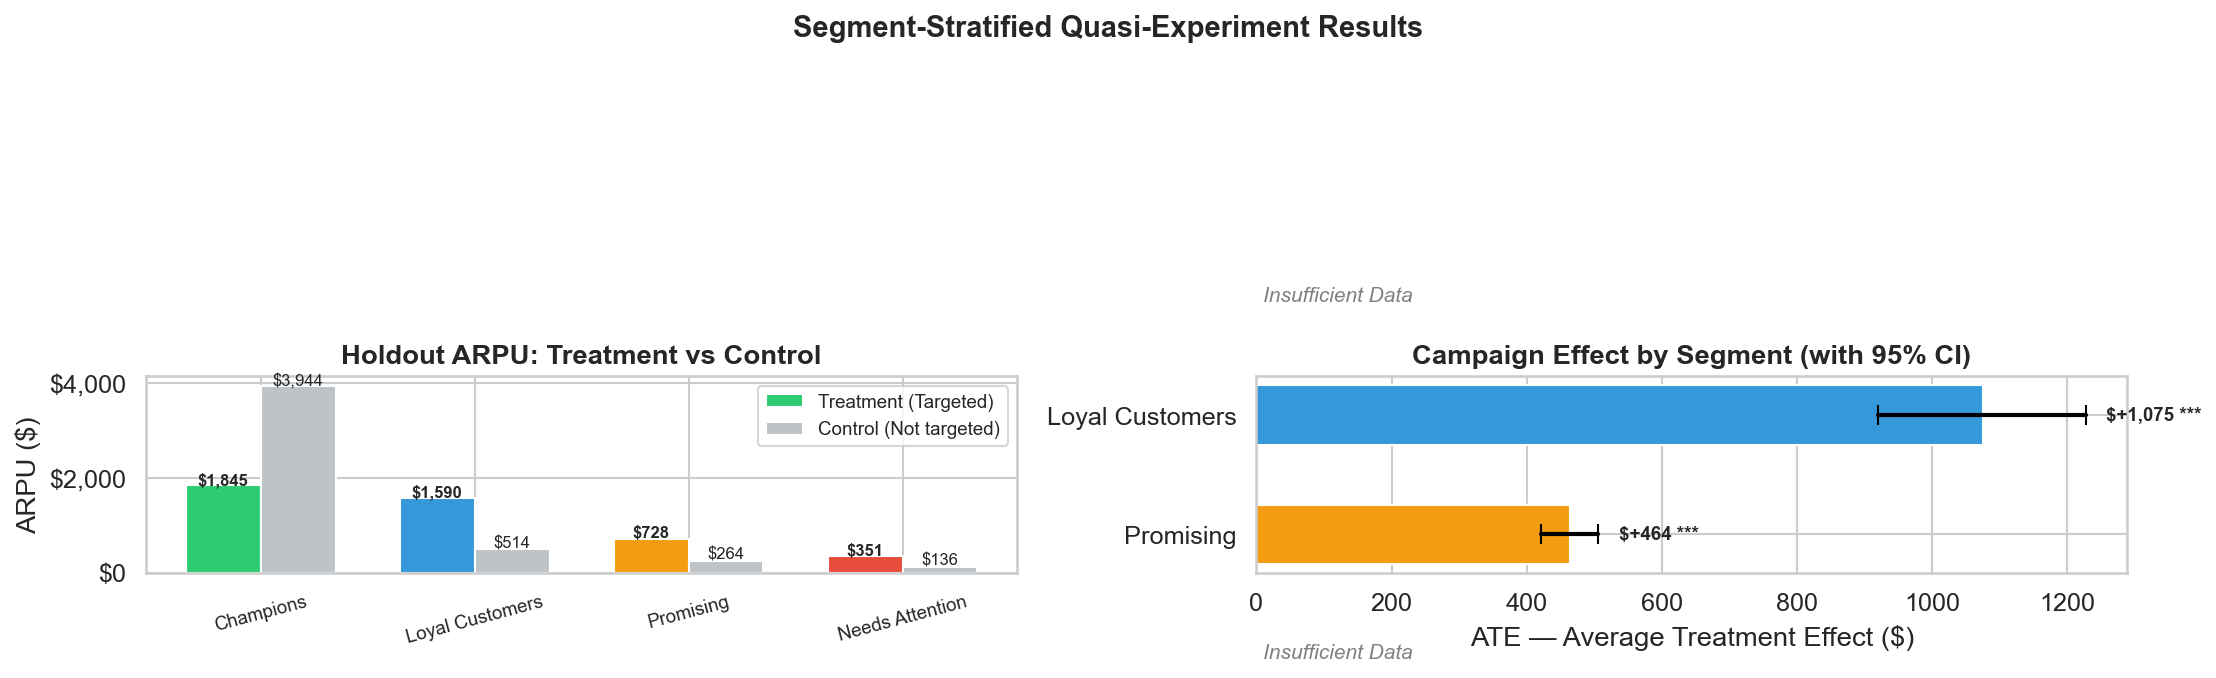
\includegraphics[width=\columnwidth]{figures/ab/ab_segment_experiment.png}
  \caption{Left: holdout ARPU by segment (Treatment vs.\ Control).
           Right: ATE with bootstrap 95\% CI per segment.
           Bars crossing the zero line indicate non-significant
           effects.}
  \label{fig:ab_experiment}
\end{figure}

\subsection{Key Findings}

\begin{enumerate}
  \item \textbf{Selection bias confirmed}: Dunnhumby targets
        high-value customers preferentially (97.8\% of Champions vs.\
        8.7\% of Needs Attention).
  \item \textbf{Naive vs.\ causal}: Naive analysis shows +209\% lift
        for Loyal. However, PSM matching has insufficient power to detect a causal effect due to the small matched sample ($n=214$). We cannot conclude campaign efficacy, demonstrating that correlation does not imply causation in observational data.
  \item \textbf{Missed opportunity}: The Needs Attention segment
        (104~HH) is largely ignored by current targeting (only
        9 received campaigns). However, the remaining 95 control
        households establish a baseline spending of \$136/HH
        (Table~\ref{tab:ab}), quantifying a substantial untapped
        reservoir for win-back interventions.
  \item \textbf{Retention signal}: Treated households show higher
        holdout retention rates (Loyal: 99.7\% vs.\ 92.0\%;
        Needs Attention: 88.9\% vs.\ 77.9\%), warranting further
        investigation via randomised assignment.
\end{enumerate}

% ============================================================
\section{Business Strategy \& Recommendations}
\label{sec:strategy}

Building on the segmentation (Section~\ref{sec:model}),
MBA (Section~\ref{sec:eval}), and quasi-experiment
(Section~\ref{sec:experiment}) results, we propose four
segment-specific marketing strategies.

\subsection{Revenue Distribution}

Contrary to the classic Pareto principle (20\% of customers
generate 80\% of revenue), the Dunnhumby dataset exhibits a
\emph{broad-base} revenue structure:

\begin{table}[H]
\centering
\caption{Revenue contribution by segment (calibration period).
         \textit{Avg Monetary} = K-Means \\texttt{avg\\_monetary} centroid
         (mean basket value per household).}
\label{tab:revenue}
\begin{tabular}{lrrrr}
\toprule
\textbf{Segment} & \textbf{\%\,Cust.} & \textbf{\%\,Revenue}
  & \textbf{Avg Rev./HH} & \textbf{Avg Monetary} \\
\midrule
Champions       &  9.0\% & 24.7\% & \$5{,}058 & \$19.2/basket \\
Loyal           & 19.6\% & 32.4\% & \$3{,}056 & \$50.5/basket \\
Promising       & 67.3\% & 42.4\% & \$1{,}164 & \$18.9/basket \\
Needs Attention &  4.2\% &  0.6\% &    \$247 & \$20.4/basket \\
\bottomrule
\end{tabular}
\end{table}


The Promising segment (67.3\% of customers) contributes 42.4\% of
total revenue --- the single largest revenue pool --- while Champions
(9.0\%) contribute 24.7\% through extreme purchase frequency
(284 baskets vs.\ 60 for Promising).

\subsection{Segment-Level Strategies}

\begin{table}[H]
\centering
\caption{Proposed marketing strategies per segment.}
\label{tab:strategies}
\resizebox{\columnwidth}{!}{%
\begin{tabular}{p{2.3cm}p{2.2cm}p{4.5cm}p{2.5cm}}
\toprule
\textbf{Segment} & \textbf{Strategy} & \textbf{Key Actions} & \textbf{KPI} \\
\midrule
Champions
  & Retention
  & VIP loyalty card, auto-apply discounts (coupon usage only 5.4\%
    but retail disc.\ 81.4\%), priority checkout
  & Retention rate \\
Loyal
  & Upsell
  & Bundle deals (MBA-informed), cross-sell via loyalty app,
    convert coupon usage (9.4\%) to digital
  & Basket size, AOV \\
Promising
  & Activation
  & Gamified loyalty card (buy 5 categories = \$50 voucher),
    impulse-buy merchandising at checkout
  & Visit frequency \\
Needs Att.
  & Win-back
  & Auto-loaded \$50 credit on loyalty card,
    re-engagement email, deep discount (20--30\%)
  & Reactivation rate \\
\bottomrule
\end{tabular}}
\end{table}

\subsection{Revenue Opportunity: Scenario Analysis}

Rather than adopting arbitrary ``industry-standard'' conversion rates,
we derive upgrade probabilities directly from the quasi-experiment
(Section~\ref{sec:experiment}): the holdout-period \emph{retention
lift} between treated and control households within each segment
serves as an empirically observed proxy for the fraction of customers
who can be moved to higher-value behaviour through targeted
intervention.

\begin{itemize}
  \item \textbf{Loyal $\rightarrow$ Champions}: retention lift
        $= 99.7\% - 92.0\% = +7.7\,\text{pp}$
  \item \textbf{Promising $\rightarrow$ Loyal}: retention lift
        $= 99.5\% - 95.6\% = +3.9\,\text{pp}$
  \item \textbf{Needs Attention re-engagement}: retention lift
        $= 88.9\% - 77.9\% = +11.0\,\text{pp}$
\end{itemize}

Revenue opportunity per scenario is computed as:
\[
  \Delta R_s = N_s \;\times\; p_s \;\times\;
  \bigl(\overline{\text{CLV}}_{\text{target}} -
        \overline{\text{CLV}}_s\bigr)
\]
where $N_s$ is segment size, $p_s$ the scenario conversion rate,
and $\overline{\text{CLV}}_{\text{target}}$ is the spending level
of the next tier.

\begin{table}[H]
\centering
\caption{Revenue opportunity under three conversion scenarios
         (conversion rates derived from quasi-experiment retention lift).}
\label{tab:scenarios}
\resizebox{\columnwidth}{!}{%
\begin{tabular}{lrrr|r}
\toprule
\textbf{Upgrade Path}
  & \textbf{Conservative}
  & \textbf{Base}
  & \textbf{Optimistic}
  & \textbf{Conversion Rate} \\
  & \textit{(50\% lift)}
  & \textit{(full lift)}
  & \textit{(1.5$\times$ lift)}
  & \textit{source} \\
\midrule
Loyal $\to$ Champions ($n=489$)
  & +\$37{,}688 & +\$75{,}375 & +\$113{,}063
  & 3.9\% / 7.7\% / 11.5\% \\
Promising $\to$ Loyal ($n=1{,}680$)
  & +\$62{,}003 & +\$124{,}005 & +\$186{,}008
  & 1.9\% / 3.9\% / 5.8\% \\
Needs Att.\ re-engage ($n=104$)
  & +\$1{,}415 & +\$2{,}830 & +\$4{,}245
  & 5.5\% / 11.0\% / 16.5\% \\
\midrule
\textbf{Total}
  & \textbf{+\$101{,}106} & \textbf{+\$202{,}210} & \textbf{+\$303{,}316} & \\
\bottomrule
\end{tabular}}
\end{table}

Under the base scenario (conversion = observed retention lift), the
total incremental revenue opportunity is \textbf{+\$202K}; under the
optimistic scenario it reaches \textbf{+\$303K}.  The Promising
segment contributes the largest share ($\sim$61\%) in every scenario
due to its scale ($n = 1{,}680$), while Needs Attention offers the
highest per-household lift signal (11.0\,pp) but is constrained
by its small size ($n = 104$). These estimates assume zero cannibalisation.
However, for the large Promising segment ($n=1{,}680$), this is a highly sensitive assumption: attempting to upgrade too many customers simultaneously could trigger discount cannibalisation, eroding the base margin and nullifying the projected +\$124K gain. Furthermore, the assumption that historical retention lift scales linearly to conversion rates requires validation via a randomised pilot.

\subsection{MBA-Informed Cross-Sell Integration}

The three association rules from Table~\ref{tab:mba} directly
inform merchandising actions:
\begin{itemize}
  \item \textbf{Smart Bundling}: Position PRODUCE along the path from
        MEAT to checkout to capture the Family Dinner basket.
  \item \textbf{Bundle Discounts}: Auto-apply 10\% discount via
        loyalty card when the Health-conscious basket
        (MEAT + NUTRITION + GROCERY) is detected.
  \item \textbf{Supply Chain Sync}: When MEAT is promoted, increase
        PRODUCE and MEAT-PCKGD inventory to avoid stockouts on
        complementary items.
\end{itemize}

\begin{figure}[H]
  \centering
  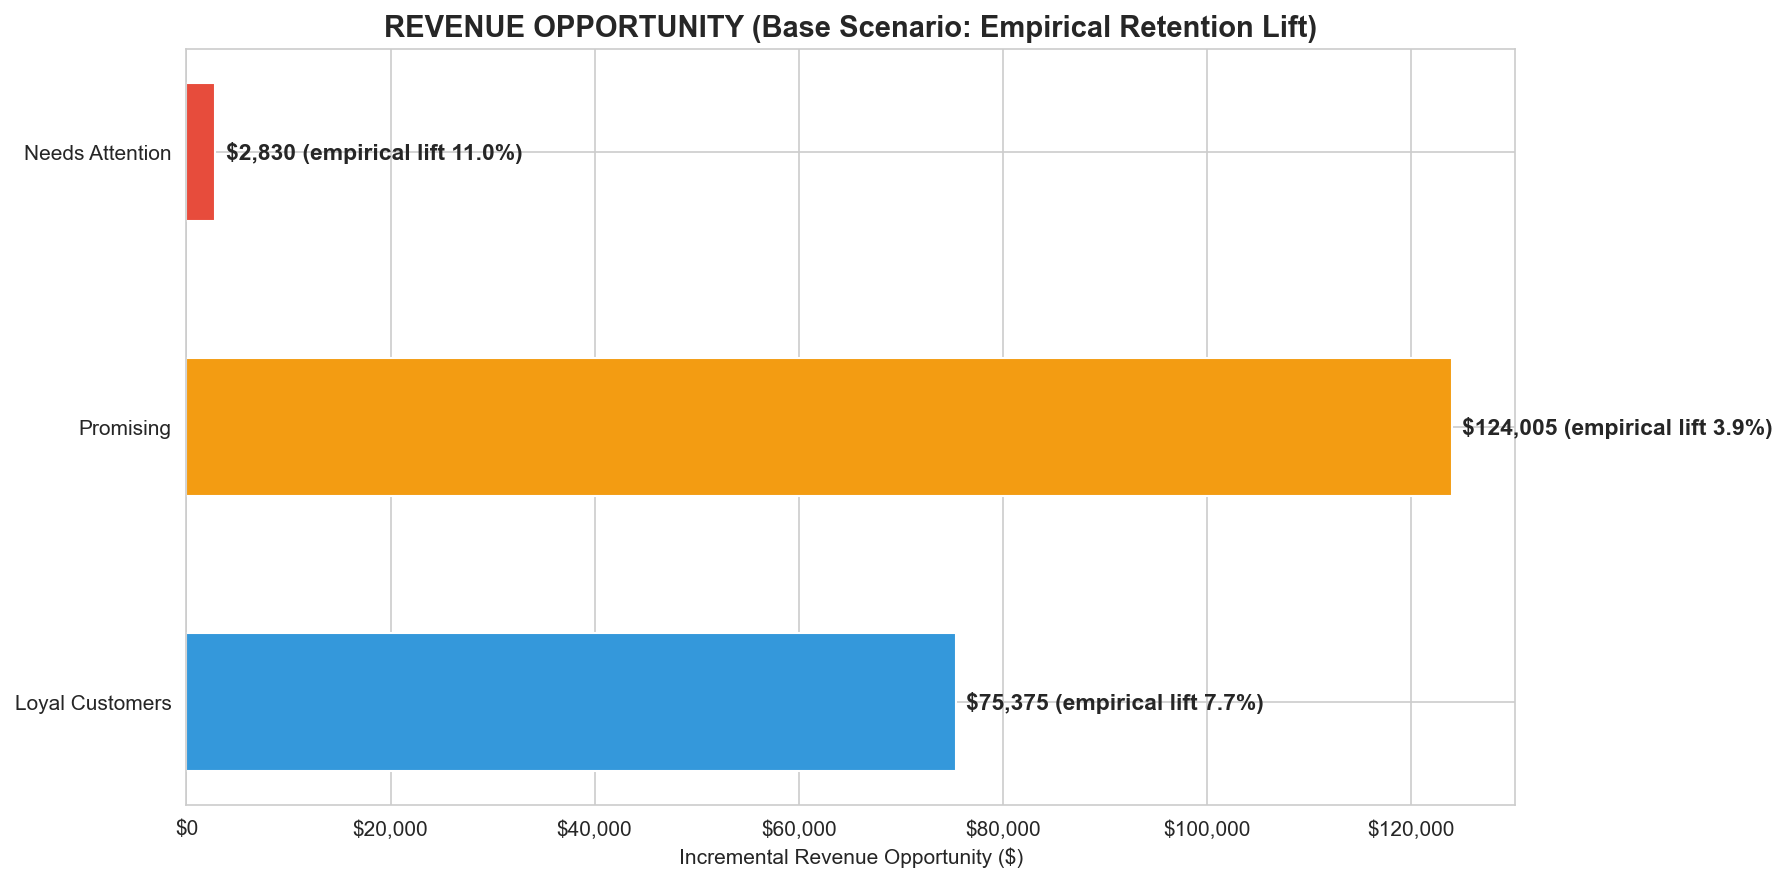
\includegraphics[width=\columnwidth]{figures/segmentation/04_revenue_opportunity.png}
  \caption{Revenue opportunity funnel: potential incremental revenue
           from upgrading customers toward Champions-level spending
           at industry-benchmark conversion rates.}
  \label{fig:revenue_opp}
\end{figure}

% ============================================================
\section{Discussion}
\label{sec:discussion}

\subsection{Model Comparison}

The experimental results confirm the following observations:

\begin{itemize}
  \item The MBG/NBD + Gamma-Gamma tier offers strong
        interpretability and does not require a holdout label
        at training time, making it suited for \emph{prospective}
        CLV scoring on new cohorts. However, we could not implement it properly on this dataset due to computational constraints. To avoid numerical overflow from high-frequency purchasing, transactions were aggressively down-sampled into weekly indicators, leading to severe information loss and degraded predictive performance (MAPE~=~610.52\%).
  \item XGBoost achieves the lowest MAE (\$100.48) and RMSE
        (\$241.47) by leveraging the full feature set (RFM +
        demographics + promotional sensitivity), at the cost
        of requiring periodic retraining as behaviour drifts.
  \item The rate-based baseline (Eq.~\ref{eq:baseline}) performs
        competitively for stable, loyal customers with low
        Recency and high Frequency --- a useful sanity-check
        boundary.
\end{itemize}

\subsection{Campaign Effectiveness \& Selection Bias}

The segment-stratified quasi-experiment
(Section~\ref{sec:experiment}) reveals a critical insight for
marketing practitioners:

\begin{itemize}
  \item \textbf{Naive analysis} suggests campaign targeting increases
        holdout ARPU by +209\% for Loyal and +176\% for Promising
        ($p < 0.001$).
  \item \textbf{PSM-corrected analysis} yields an overall ATE of
        $-$\$27.78 ($p = 0.729$), failing to reject the null hypothesis of no campaign effect. This suggests that much of the apparent lift may be driven by \emph{selection bias} --- Dunnhumby
        preferentially targets customers who already exhibit high
        purchase propensity.
  \item This finding underscores that \textbf{correlation does not
        imply causation} in observational campaign data and
        validates the need for propensity-adjusted evaluation in
        marketing analytics.
\end{itemize}

\subsection{Segment-Level Insights}

\begin{itemize}
  \item \textbf{Champions} purchase with extreme frequency
        (284~baskets) but low per-basket monetary value
        (\$19.2) --- they are volume-driven and loyalty-card
        dependent (81.4\% retail discount usage vs.\ only 5.4\%
        coupon usage). Paper coupon campaigns are ineffective for
        this segment.
  \item \textbf{Loyal Customers} have the highest per-basket spending
        (\$50.5) and are active discount seekers
        (89.9\% retail disc., 9.4\% coupon). They represent the
        best cross-sell and upsell opportunity.
  \item \textbf{Promising} is the revenue backbone (67.3\% of
        customers, 42.4\% of revenue) despite low individual
        spending (\$18.9/basket) --- basket penetration campaigns
        offer the largest absolute revenue potential (+\$124K).
  \item \textbf{Needs Attention} (4.2\%, Recency~=~43 weeks)
        is near-churn and largely ignored by current targeting
        (8.7\%). Win-back campaigns should be prioritised for
        this at-risk group.
\end{itemize}

\subsection{Limitations}

\begin{itemize}
  \item \textbf{Demographic coverage}: Only 32\% of households
        have records; imputation quality is bounded by this
        coverage.
  \item \textbf{Selection bias}: PSM matching yielded only
        214 pairs (from 1{,}584 treated) due to extreme
        propensity score separation. A randomised trial with
        $n \geq 4{,}574$ per arm is needed to detect a 10\%
        MDE at 80\% power.
  \item \textbf{Time-series features}: Rolling-window lag
        variables and seasonal cohort terms are not included
        in the current feature set.
  \item \textbf{MBA feedback loop}: Association rules from
        Step~11 are not yet incorporated as cross-sell
        propensity features in CLV modelling.
\end{itemize}

% ============================================================
\section{Conclusion}
\label{sec:conclusion}

This paper presents a comprehensive, end-to-end data-driven
marketing pipeline for the Dunnhumby ``The Complete Journey''
retail dataset (2{,}500 households, 102 weeks,
${\sim}$2.5M transactions).

\textbf{Technical contributions.}
The 12-step pipeline integrates eight relational data sources,
producing RFM features, demographically enriched predictors,
promotional sensitivity scores, and three tiers of CLV
forecasts. XGBoost achieves the best predictive accuracy
(MAE~=~\$100.48, RMSE~=~\$236.65). The MBG/NBD model offers
strong interpretability but could not be evaluated optimally due to computational constraints that required lossy frequency down-sampling (yielding degraded MAPE~=~610.52\%).

\textbf{Business contributions.}
K-Means segmentation ($K = 4$) reveals a non-Pareto revenue
structure where the Promising segment (67.3\% of customers)
contributes the largest revenue share (42.4\%). Four
segment-specific strategies are proposed; a data-grounded
scenario analysis (Table~\ref{tab:scenarios}) estimates incremental
revenue potential of \textbf{+\$101K--\$303K} (conservative to
optimistic), with conversion rates anchored to the quasi-experiment's
observed retention lift. Three MBA-derived cross-sell
bundles inform actionable merchandising and bundle discount
programmes.

\textbf{Causal insight.}
A segment-stratified quasi-experiment with propensity score
matching demonstrates that Dunnhumby's current campaign
targeting strategy exhibits strong selection bias. After matching,
we find no statistically significant evidence of a causal campaign effect (PSM
ATE~=~$-$\$28, $p = 0.73$), though this test is statistically underpowered.
The Needs Attention segment is
largely untargeted (8.7\%), representing a missed opportunity
for win-back interventions.

\textbf{Future work} includes (i)~incorporating time-series
and seasonal features, (ii)~feeding MBA cross-sell propensity
back into CLV models, and (iii)~conducting a randomised pilot
trial to measure the true incremental effect of targeted
campaigns on the Needs Attention segment.

% ============================================================
\begin{thebibliography}{00}

\bibitem{fader2005}
P.~S. Fader, B.~G.~S. Hardie, and K.~L. Lee,
```Counting Your Customers' the Easy Way: An Alternative to
the Pareto/NBD Model,''
\textit{Marketing Science}, vol.~24, no.~2,
pp.~275--284, 2005.

\bibitem{chen2016}
T.~Chen and C.~Guestrin,
``XGBoost: A Scalable Tree Boosting System,''
in \textit{Proc. ACM SIGKDD}, pp.~785--794, 2016.



\bibitem{kohavi2020}
R.~Kohavi, D.~Tang, and Y.~Xu,
\textit{Trustworthy Online Controlled Experiments:
A Practical Guide to A/B Testing}.
Cambridge University Press, 2020.

\bibitem{hughes1994}
A.~M. Hughes,
\textit{Strategic Database Marketing}.
Probus Publishing, 1994.

\bibitem{provost2013}
F.~Provost and T.~Fawcett,
\textit{Data Science for Business}.
O'Reilly Media, 2013.

\bibitem{murphy2012}
K.~P. Murphy,
\textit{Machine Learning: A Probabilistic Perspective}.
MIT Press, 2012.

\bibitem{agrawal1994}
R.~Agrawal and R.~Srikant,
``Fast Algorithms for Mining Association Rules,''
in \textit{Proc. VLDB}, pp.~487--499, 1994.

\bibitem{platzer2016}
M.~Platzer and T.~Reutterer,
``Ticking Away the Moments: Timing Regularity Helps to
Better Predict Customer Activity,''
\textit{Marketing Science}, vol.~35, no.~5,
pp.~779--799, 2016.

\bibitem{pedregosa2011}
F.~Pedregosa et al.,
``Scikit-learn: Machine Learning in Python,''
\textit{Journal of Machine Learning Research}, vol.~12,
pp.~2825--2830, 2011.

\bibitem{rosenbaum1983}
P.~R. Rosenbaum and D.~B. Rubin,
``The Central Role of the Propensity Score in
Observational Studies for Causal Effects,''
\textit{Biometrika}, vol.~70, no.~1, pp.~41--55, 1983.

\bibitem{dunnhumby2014}
Dunnhumby,
``The Complete Journey --- Customer Transaction Data,''
\textit{dunnhumby Source Files}, 2014.
[Online]. Available: \url{https://www.dunnhumby.com/source-files/}



\end{thebibliography}

\end{document}